\subsection{PTIME (PSPACE)}
Třída všech problémů, které lze řešit algoritmy s \textbf{polynomiální časovou (prostorovou) složitosti}, tj. s časovou složitosti $O (n^k)$, kde $k$ je nějaká konstanta. 

Tuto třídu problému považujeme za zvládnutelnou. Je \textbf{robustní} -- mezi jednotlivými výpočetními modely (RAM, TS) existují vzájemné polynominální simulace, nezáleží tedy jakým modelem budeme algoritmus simulovat, vždy bude patřit do třídy PTIME.
\subsubsection{Problémy pařící do třídy PTIME}
\begin{itemize}
\item Třídění a vyhledávání.
\item Nejkratší cesta v grafu
a minimální kostra grafu.
\item Ekvivalence deterministických konečných automatů.
\item Přijatelnost slova bezkontextovou gramatikou.
\end{itemize}


\begin{enumerate}
\item \textbf{Výběr aktivit}
\begin{itemize}
	\item \textbf{\textsc{Vstup}}: Množina aktivit s časovými intervaly, kdy je lze vykonávat.
	\item \textbf{\textsc{Výstup}}: Největší možný počet kompatibilních aktivit (aktivit, které se nekryjí).
\end{itemize}
\item \textbf{Optimalizace násobení řetězce matic}
\begin{itemize}
	\item \textbf{\textsc{Vstup}}: Posloupnost matic.
	\item \textbf{\textsc{Výstup}}: Plně uzávorkovaný součin.
\end{itemize}
\item \textbf{LCS - problém nejdelší společné posloupnosti}
\begin{itemize}
	\item \textbf{\textsc{Vstup}}: Dvě posloupnosti $v,w$ v nějaké abecedě $\Sigma$.
	\item \textbf{\textsc{Výstup}}: Nejdelší společná podposloupnost posloupností $v,w$.
\end{itemize}
\end{enumerate}

\subsection{NPTIME}
Třída všech rozhodovacích problémů (ano/ne), které jsou rozhodovány \textbf{nedeterministickými algoritmy s polynomiální časovou složitosti}.

Pokud je odpověď ANO, tak stačí nalézt jedno řešení s touto odpovědí. Pokud je odpověď NE, je potřeba ukázat, že žádné řešení nevrací ANO.

\subsection{Třída NP-úplných problémů}
NP-úplné problémy jsou takové problémy, na které jsou \textbf{polynomiálně redukovatelné všechny ostatní problémy z třídy NP}. To znamená, že třídu NP-úplných úloh tvoří v jistém smyslu ty \textbf{nejtěžší úlohy} z NP. 

Pokud by byl nalezen deterministický polynomiální algoritmus pro nějakou NP-úplnou úlohu, znamenalo by to, že všechny nedeterministicky polynomiální problémy jsou řešitelné v polynomiálním čase (tedy že NP = P). Otázka, zda nějaký takový algoritmus existuje, zatím nebyla rozhodnuta, předpokládá se však, že NP $\neq$ P (\textbf{je však zřejmé, že P $\subseteq$ NP}).

\begin{figure}[H]
	\centering
	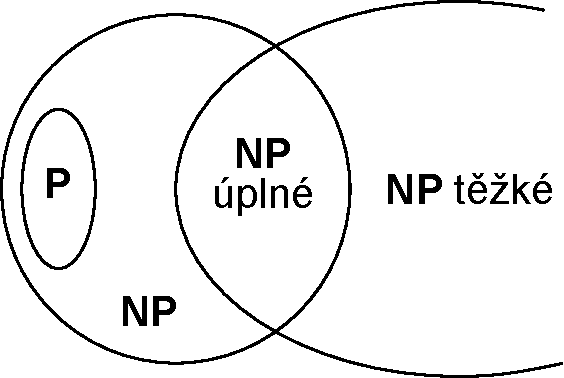
\includegraphics[width=0.4\textwidth]{assets/np_problemy}
\end{figure}

\subsubsection{NP-těžký problém}
Problém $P$ nazveme NP-těžkým, pokud pro \textbf{libovolný problém} $A$ ze třídy NP platí, že $A$ je \textbf{polynominálně převeditelné} (redukovatelné) na problém $P$, tedy pokud platí:
$\forall P \in \textrm{NPTIME}: P \triangleright Q$.

\subsubsection{NP-úplný problém}
Třída nejtěžších NPTIME problémů. Problém P je NP-úplný, pokud patří do třídy \textbf{NP} a je \textbf{NP-těžký}.

\subsubsection{NP-úplné problémy}

\begin{enumerate}
	\item \textbf{IS (problém nezávislé množiny)}
	\begin{itemize}
		\item \textbf{\textsc{Vstup}}: Neorientovaný graf $G$ (o $n$ vrcholech), číslo $k$ ($k \leq n$).
		\item \textbf{\textsc{Otázka}}: Existuje v $G$ nezávislá množina velikosti $k$ (tj. množina $k$ vrcholů, z nichž žádné dva nejsou spojeny hranou)?
		\begin{figure}[H]
			\centering
			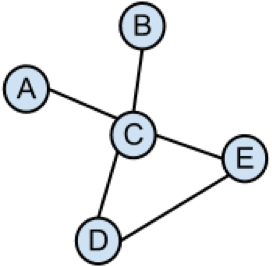
\includegraphics[width=0.15\textwidth]{assets/problem_is}
		\end{figure}
		Program vybere náhodně $k$ vrcholů z grafu a ověří zdali nejsou některé spojeny hranou. Když mezi nimi hranu \textbf{nenajde}, vrátí odpověď \textit{,,ANO, v grafu existuje nezávislá množina o velikosti $k$''}. Když hranu mezi zvolenou množinou \textbf{najde}, vrátí odpověď ,,NE''. Přičemž odpověď ne \textbf{může být chybná}.
		\\\\
		\textbf{Výstup} pro $k > 3$: NE.
\\
		\textbf{Výstup} pro $k = 3$: ANO (ABD, ABE).
\\
		\textbf{Výstup} pro $k = 2$: ANO (AB, AD, AE, BD, BE).
	\end{itemize}
	\item \textbf{Isomorfismus grafů}
	\begin{itemize}
		\item \textbf{\textsc{Vstup}}: Dva neorientované grafy $ G $ a $ H $.
		\item \textbf{\textsc{Otázka}}: Jsou grafy $ G $ a $ H $ izomorfní?
	\end{itemize}
	\item \textbf{CG (Barvení grafu)}
	\begin{itemize}
		\item \textbf{\textsc{Vstup}}: Neorientovaný graf $ G $ a číslo $ k $.
		\item \textbf{\textsc{Otázka}}: Je možné graf $ G $ obarvit $ k $ barvami (tj. existuje přiřazení barev vrcholům tak, aby žádné dva sousední vrcholy nebyly obarveny stejnou barvou)?
	\end{itemize}
	\item \textbf{SAT (problém splnitelnosti booleovských formulí)}
	\begin{itemize}
		\item \textbf{\textsc{Vstup}}: Booleovská formule v konjunktivní normální formě.
		\item \textbf{\textsc{Otázka}}: Je daná formule splnitelná (tj. existuje pravdivostní ohodnocení proměnných, při kterém je formule pravdivá)?
	\end{itemize}
	\item \textbf{3-SAT (problém SAT s omezením na 3 literály)}
	\begin{itemize}
		\item \textbf{\textsc{Vstup}}: Formule v konjunktivní normální formě, kde každá klauzule obsahuje pravě 3 literály.
		\item \textbf{\textsc{Otázka}}: Je formule splnitelná?
	\end{itemize}
	\item \textbf{HK (problém hamiltonovské kružnice)/HC (problém hamiltonovskho cyklu) }
	\begin{itemize}
		\item \textbf{\textsc{Vstup}}: Neorientovaný graf $ G $/Orientovaný grav $ G $.
		\item \textbf{\textsc{Otázka}}: Existuje v $ G $ hamiltonovská kružnice (uzavřená cesta, procházející každým vrcholem právě jednou)?
	\end{itemize}
	\item \textbf{Subset-Sum}
	\begin{itemize}
		\item \textbf{\textsc{Vstup}}: Množina přirozených čísel $ M = {x_1, x_2, \ldots, x_n} $ a přirozené číslo $ s $.
		\item \textbf{\textsc{Otázka}}: Existuje podmnožina množiny $ M $, pro niž součet jejích prvků je roven $ s $?
	\end{itemize}
	\item \textbf{Problém obchodního cestujícího (TSP) ANO/NE verze}
	\begin{itemize}
		\item \textbf{\textsc{Vstup}}: Neorientovaný graf $ G $ s hranami ohodnocenými přirozenými čísly a číslo $ k $.
		\item \textbf{\textsc{Otázka}}: lze objet $k$ měst a neujet víc než danou vzdálenost?
	\end{itemize}
	\item \textbf{Vrcholové pokryti (vertex cover)}
	\begin{itemize}
		\item \textbf{\textsc{Vstup}}: Neorientovaný graf $ G $ a přirozené číslo $ k $.
		\item \textbf{\textsc{Otázka}}: Existuje v grafu $ G $ množina vrcholů velikosti $ k $ taková, že každá hrana má alespoň jeden svůj vrchol v teto množině?
	\end{itemize}
\end{enumerate}